% Options for packages loaded elsewhere
\PassOptionsToPackage{unicode}{hyperref}
\PassOptionsToPackage{hyphens}{url}
%
\documentclass[
]{article}
\usepackage{lmodern}
\usepackage{amssymb,amsmath}
\usepackage{ifxetex,ifluatex}
\ifnum 0\ifxetex 1\fi\ifluatex 1\fi=0 % if pdftex
  \usepackage[T1]{fontenc}
  \usepackage[utf8]{inputenc}
  \usepackage{textcomp} % provide euro and other symbols
\else % if luatex or xetex
  \usepackage{unicode-math}
  \defaultfontfeatures{Scale=MatchLowercase}
  \defaultfontfeatures[\rmfamily]{Ligatures=TeX,Scale=1}
\fi
% Use upquote if available, for straight quotes in verbatim environments
\IfFileExists{upquote.sty}{\usepackage{upquote}}{}
\IfFileExists{microtype.sty}{% use microtype if available
  \usepackage[]{microtype}
  \UseMicrotypeSet[protrusion]{basicmath} % disable protrusion for tt fonts
}{}
\makeatletter
\@ifundefined{KOMAClassName}{% if non-KOMA class
  \IfFileExists{parskip.sty}{%
    \usepackage{parskip}
  }{% else
    \setlength{\parindent}{0pt}
    \setlength{\parskip}{6pt plus 2pt minus 1pt}}
}{% if KOMA class
  \KOMAoptions{parskip=half}}
\makeatother
\usepackage{xcolor}
\IfFileExists{xurl.sty}{\usepackage{xurl}}{} % add URL line breaks if available
\IfFileExists{bookmark.sty}{\usepackage{bookmark}}{\usepackage{hyperref}}
\hypersetup{
  pdftitle={Flujo de análisis en clasificación supervisada},
  pdfauthor={Laura Rodríguez Navas},
  hidelinks,
  pdfcreator={LaTeX via pandoc}}
\urlstyle{same} % disable monospaced font for URLs
\usepackage[margin=1in]{geometry}
\usepackage{color}
\usepackage{fancyvrb}
\newcommand{\VerbBar}{|}
\newcommand{\VERB}{\Verb[commandchars=\\\{\}]}
\DefineVerbatimEnvironment{Highlighting}{Verbatim}{commandchars=\\\{\}}
% Add ',fontsize=\small' for more characters per line
\usepackage{framed}
\definecolor{shadecolor}{RGB}{248,248,248}
\newenvironment{Shaded}{\begin{snugshade}}{\end{snugshade}}
\newcommand{\AlertTok}[1]{\textcolor[rgb]{0.94,0.16,0.16}{#1}}
\newcommand{\AnnotationTok}[1]{\textcolor[rgb]{0.56,0.35,0.01}{\textbf{\textit{#1}}}}
\newcommand{\AttributeTok}[1]{\textcolor[rgb]{0.77,0.63,0.00}{#1}}
\newcommand{\BaseNTok}[1]{\textcolor[rgb]{0.00,0.00,0.81}{#1}}
\newcommand{\BuiltInTok}[1]{#1}
\newcommand{\CharTok}[1]{\textcolor[rgb]{0.31,0.60,0.02}{#1}}
\newcommand{\CommentTok}[1]{\textcolor[rgb]{0.56,0.35,0.01}{\textit{#1}}}
\newcommand{\CommentVarTok}[1]{\textcolor[rgb]{0.56,0.35,0.01}{\textbf{\textit{#1}}}}
\newcommand{\ConstantTok}[1]{\textcolor[rgb]{0.00,0.00,0.00}{#1}}
\newcommand{\ControlFlowTok}[1]{\textcolor[rgb]{0.13,0.29,0.53}{\textbf{#1}}}
\newcommand{\DataTypeTok}[1]{\textcolor[rgb]{0.13,0.29,0.53}{#1}}
\newcommand{\DecValTok}[1]{\textcolor[rgb]{0.00,0.00,0.81}{#1}}
\newcommand{\DocumentationTok}[1]{\textcolor[rgb]{0.56,0.35,0.01}{\textbf{\textit{#1}}}}
\newcommand{\ErrorTok}[1]{\textcolor[rgb]{0.64,0.00,0.00}{\textbf{#1}}}
\newcommand{\ExtensionTok}[1]{#1}
\newcommand{\FloatTok}[1]{\textcolor[rgb]{0.00,0.00,0.81}{#1}}
\newcommand{\FunctionTok}[1]{\textcolor[rgb]{0.00,0.00,0.00}{#1}}
\newcommand{\ImportTok}[1]{#1}
\newcommand{\InformationTok}[1]{\textcolor[rgb]{0.56,0.35,0.01}{\textbf{\textit{#1}}}}
\newcommand{\KeywordTok}[1]{\textcolor[rgb]{0.13,0.29,0.53}{\textbf{#1}}}
\newcommand{\NormalTok}[1]{#1}
\newcommand{\OperatorTok}[1]{\textcolor[rgb]{0.81,0.36,0.00}{\textbf{#1}}}
\newcommand{\OtherTok}[1]{\textcolor[rgb]{0.56,0.35,0.01}{#1}}
\newcommand{\PreprocessorTok}[1]{\textcolor[rgb]{0.56,0.35,0.01}{\textit{#1}}}
\newcommand{\RegionMarkerTok}[1]{#1}
\newcommand{\SpecialCharTok}[1]{\textcolor[rgb]{0.00,0.00,0.00}{#1}}
\newcommand{\SpecialStringTok}[1]{\textcolor[rgb]{0.31,0.60,0.02}{#1}}
\newcommand{\StringTok}[1]{\textcolor[rgb]{0.31,0.60,0.02}{#1}}
\newcommand{\VariableTok}[1]{\textcolor[rgb]{0.00,0.00,0.00}{#1}}
\newcommand{\VerbatimStringTok}[1]{\textcolor[rgb]{0.31,0.60,0.02}{#1}}
\newcommand{\WarningTok}[1]{\textcolor[rgb]{0.56,0.35,0.01}{\textbf{\textit{#1}}}}
\usepackage{graphicx,grffile}
\makeatletter
\def\maxwidth{\ifdim\Gin@nat@width>\linewidth\linewidth\else\Gin@nat@width\fi}
\def\maxheight{\ifdim\Gin@nat@height>\textheight\textheight\else\Gin@nat@height\fi}
\makeatother
% Scale images if necessary, so that they will not overflow the page
% margins by default, and it is still possible to overwrite the defaults
% using explicit options in \includegraphics[width, height, ...]{}
\setkeys{Gin}{width=\maxwidth,height=\maxheight,keepaspectratio}
% Set default figure placement to htbp
\makeatletter
\def\fps@figure{htbp}
\makeatother
\setlength{\emergencystretch}{3em} % prevent overfull lines
\providecommand{\tightlist}{%
  \setlength{\itemsep}{0pt}\setlength{\parskip}{0pt}}
\setcounter{secnumdepth}{5}

\title{Flujo de análisis en clasificación supervisada}
\usepackage{etoolbox}
\makeatletter
\providecommand{\subtitle}[1]{% add subtitle to \maketitle
  \apptocmd{\@title}{\par {\large #1 \par}}{}{}
}
\makeatother
\subtitle{Métodos supervisados}
\author{Laura Rodríguez Navas}
\date{Septiembre 2020}

\begin{document}
\maketitle

{
\setcounter{tocdepth}{2}
\tableofcontents
}
Comenzamos cargando los paquetes y la base de datos:

\begin{Shaded}
\begin{Highlighting}[]
\KeywordTok{library}\NormalTok{(caret)}
\KeywordTok{library}\NormalTok{(mlbench)}
\KeywordTok{data}\NormalTok{(Sonar)}
\KeywordTok{str}\NormalTok{(Sonar, }\DataTypeTok{width =} \DecValTok{85}\NormalTok{, }\DataTypeTok{strict.width =} \StringTok{"cut"}\NormalTok{)}
\end{Highlighting}
\end{Shaded}

\begin{verbatim}
## 'data.frame':    208 obs. of  61 variables:
##  $ V1   : num  0.02 0.0453 0.0262 0.01 0.0762 0.0286 0.0317 0.0519 0.0223 0.0164 ...
##  $ V2   : num  0.0371 0.0523 0.0582 0.0171 0.0666 0.0453 0.0956 0.0548 0.0375 0.017..
##  $ V3   : num  0.0428 0.0843 0.1099 0.0623 0.0481 ...
##  $ V4   : num  0.0207 0.0689 0.1083 0.0205 0.0394 ...
##  $ V5   : num  0.0954 0.1183 0.0974 0.0205 0.059 ...
##  $ V6   : num  0.0986 0.2583 0.228 0.0368 0.0649 ...
##  $ V7   : num  0.154 0.216 0.243 0.11 0.121 ...
##  $ V8   : num  0.16 0.348 0.377 0.128 0.247 ...
##  $ V9   : num  0.3109 0.3337 0.5598 0.0598 0.3564 ...
##  $ V10  : num  0.211 0.287 0.619 0.126 0.446 ...
##  $ V11  : num  0.1609 0.4918 0.6333 0.0881 0.4152 ...
##  $ V12  : num  0.158 0.655 0.706 0.199 0.395 ...
##  $ V13  : num  0.2238 0.6919 0.5544 0.0184 0.4256 ...
##  $ V14  : num  0.0645 0.7797 0.532 0.2261 0.4135 ...
##  $ V15  : num  0.066 0.746 0.648 0.173 0.453 ...
##  $ V16  : num  0.227 0.944 0.693 0.213 0.533 ...
##  $ V17  : num  0.31 1 0.6759 0.0693 0.7306 ...
##  $ V18  : num  0.3 0.887 0.755 0.228 0.619 ...
##  $ V19  : num  0.508 0.802 0.893 0.406 0.203 ...
##  $ V20  : num  0.48 0.782 0.862 0.397 0.464 ...
##  $ V21  : num  0.578 0.521 0.797 0.274 0.415 ...
##  $ V22  : num  0.507 0.405 0.674 0.369 0.429 ...
##  $ V23  : num  0.433 0.396 0.429 0.556 0.573 ...
##  $ V24  : num  0.555 0.391 0.365 0.485 0.54 ...
##  $ V25  : num  0.671 0.325 0.533 0.314 0.316 ...
##  $ V26  : num  0.641 0.32 0.241 0.533 0.229 ...
##  $ V27  : num  0.71 0.327 0.507 0.526 0.7 ...
##  $ V28  : num  0.808 0.277 0.853 0.252 1 ...
##  $ V29  : num  0.679 0.442 0.604 0.209 0.726 ...
##  $ V30  : num  0.386 0.203 0.851 0.356 0.472 ...
##  $ V31  : num  0.131 0.379 0.851 0.626 0.51 ...
##  $ V32  : num  0.26 0.295 0.504 0.734 0.546 ...
##  $ V33  : num  0.512 0.198 0.186 0.612 0.288 ...
##  $ V34  : num  0.7547 0.2341 0.2709 0.3497 0.0981 ...
##  $ V35  : num  0.854 0.131 0.423 0.395 0.195 ...
##  $ V36  : num  0.851 0.418 0.304 0.301 0.418 ...
##  $ V37  : num  0.669 0.384 0.612 0.541 0.46 ...
##  $ V38  : num  0.61 0.106 0.676 0.881 0.322 ...
##  $ V39  : num  0.494 0.184 0.537 0.986 0.283 ...
##  $ V40  : num  0.274 0.197 0.472 0.917 0.243 ...
##  $ V41  : num  0.051 0.167 0.465 0.612 0.198 ...
##  $ V42  : num  0.2834 0.0583 0.2587 0.5006 0.2444 ...
##  $ V43  : num  0.282 0.14 0.213 0.321 0.185 ...
##  $ V44  : num  0.4256 0.1628 0.2222 0.3202 0.0841 ...
##  $ V45  : num  0.2641 0.0621 0.2111 0.4295 0.0692 ...
##  $ V46  : num  0.1386 0.0203 0.0176 0.3654 0.0528 ...
##  $ V47  : num  0.1051 0.053 0.1348 0.2655 0.0357 ...
##  $ V48  : num  0.1343 0.0742 0.0744 0.1576 0.0085 ...
##  $ V49  : num  0.0383 0.0409 0.013 0.0681 0.023 0.0264 0.0507 0.0285 0.0777 0.0092 ..
##  $ V50  : num  0.0324 0.0061 0.0106 0.0294 0.0046 0.0081 0.0159 0.0178 0.0439 0.019..
##  $ V51  : num  0.0232 0.0125 0.0033 0.0241 0.0156 0.0104 0.0195 0.0052 0.0061 0.011..
##  $ V52  : num  0.0027 0.0084 0.0232 0.0121 0.0031 0.0045 0.0201 0.0081 0.0145 0.009..
##  $ V53  : num  0.0065 0.0089 0.0166 0.0036 0.0054 0.0014 0.0248 0.012 0.0128 0.0223..
##  $ V54  : num  0.0159 0.0048 0.0095 0.015 0.0105 0.0038 0.0131 0.0045 0.0145 0.0179..
##  $ V55  : num  0.0072 0.0094 0.018 0.0085 0.011 0.0013 0.007 0.0121 0.0058 0.0084 ...
##  $ V56  : num  0.0167 0.0191 0.0244 0.0073 0.0015 0.0089 0.0138 0.0097 0.0049 0.006..
##  $ V57  : num  0.018 0.014 0.0316 0.005 0.0072 0.0057 0.0092 0.0085 0.0065 0.0032 ...
##  $ V58  : num  0.0084 0.0049 0.0164 0.0044 0.0048 0.0027 0.0143 0.0047 0.0093 0.003..
##  $ V59  : num  0.009 0.0052 0.0095 0.004 0.0107 0.0051 0.0036 0.0048 0.0059 0.0056 ..
##  $ V60  : num  0.0032 0.0044 0.0078 0.0117 0.0094 0.0062 0.0103 0.0053 0.0022 0.004..
##  $ Class: Factor w/ 2 levels "M","R": 2 2 2 2 2 2 2 2 2 2 ...
\end{verbatim}

La base de datos \emph{Sonar}, con 208 instancias, contiene 60 variables
explicativas numéricas y dos valores en la variable clase (``M'' y
``R'').

Definimos las instancias de train y test que darán forma al modelo de
clasificación. Fijamos una semilla para futuras generaciones de números
aleatorios. Hacemos uso de la función \textbf{createDataPartition} para
generar una partición train-test de las 208 instancias, que mantendremos
durante todo el flujo de análisis.

Tomaremos una muestra del 75\% de la base de datos como conjunto de
datos de train, y el 25\% de la misma como conjunto de datos de test.

\begin{Shaded}
\begin{Highlighting}[]
\KeywordTok{set.seed}\NormalTok{(}\DecValTok{107}\NormalTok{)}
\NormalTok{inTrain <-}\StringTok{ }\KeywordTok{createDataPartition}\NormalTok{(}\DataTypeTok{y=}\NormalTok{Sonar}\OperatorTok{$}\NormalTok{Class, }\DataTypeTok{p=}\NormalTok{.}\DecValTok{75}\NormalTok{, }\DataTypeTok{list=}\OtherTok{FALSE}\NormalTok{)}
\NormalTok{training <-}\StringTok{ }\NormalTok{Sonar[inTrain, ]}
\NormalTok{testing <-}\StringTok{ }\NormalTok{Sonar[}\OperatorTok{-}\NormalTok{inTrain, ]}
\end{Highlighting}
\end{Shaded}

El conjunto de datos de train contiene 157 instancias y el conjunto de
datos de test contiene 51 instancias.

\begin{Shaded}
\begin{Highlighting}[]
\KeywordTok{dim}\NormalTok{(training)}
\end{Highlighting}
\end{Shaded}

\begin{verbatim}
## [1] 157  61
\end{verbatim}

\begin{Shaded}
\begin{Highlighting}[]
\KeywordTok{dim}\NormalTok{(testing)}
\end{Highlighting}
\end{Shaded}

\begin{verbatim}
## [1] 51 61
\end{verbatim}

El mismo proceso usando la función \textbf{createFolds}.

\begin{Shaded}
\begin{Highlighting}[]
\KeywordTok{set.seed}\NormalTok{(}\DecValTok{107}\NormalTok{)}
\NormalTok{folds <-}\StringTok{ }\KeywordTok{createFolds}\NormalTok{(}\DataTypeTok{y=}\NormalTok{Sonar}\OperatorTok{$}\NormalTok{Class, }\DataTypeTok{k=}\DecValTok{10}\NormalTok{, }\DataTypeTok{list=}\OtherTok{TRUE}\NormalTok{, }\DataTypeTok{returnTrain =} \OtherTok{TRUE}\NormalTok{)}
\KeywordTok{lapply}\NormalTok{(folds, length)}
\end{Highlighting}
\end{Shaded}

\begin{verbatim}
## $Fold01
## [1] 188
## 
## $Fold02
## [1] 186
## 
## $Fold03
## [1] 187
## 
## $Fold04
## [1] 188
## 
## $Fold05
## [1] 188
## 
## $Fold06
## [1] 187
## 
## $Fold07
## [1] 187
## 
## $Fold08
## [1] 187
## 
## $Fold09
## [1] 187
## 
## $Fold10
## [1] 187
\end{verbatim}

\begin{Shaded}
\begin{Highlighting}[]
\NormalTok{fold <-}\StringTok{ }\NormalTok{folds[[}\DecValTok{1}\NormalTok{]]}
\NormalTok{training_folds <-}\StringTok{ }\NormalTok{Sonar[fold, ]}
\NormalTok{testing_folds <-}\StringTok{ }\NormalTok{Sonar[}\OperatorTok{-}\NormalTok{fold, ]}
\end{Highlighting}
\end{Shaded}

El conjunto de datos de train contiene 188 instancias y el conjunto de
datos de test contiene 20 instancias.

\begin{Shaded}
\begin{Highlighting}[]
\KeywordTok{dim}\NormalTok{(training_folds)}
\end{Highlighting}
\end{Shaded}

\begin{verbatim}
## [1] 188  61
\end{verbatim}

\begin{Shaded}
\begin{Highlighting}[]
\KeywordTok{dim}\NormalTok{(testing_folds)}
\end{Highlighting}
\end{Shaded}

\begin{verbatim}
## [1] 20 61
\end{verbatim}

Usamos la función \textbf{createResample}.

\begin{Shaded}
\begin{Highlighting}[]
\KeywordTok{set.seed}\NormalTok{(}\DecValTok{107}\NormalTok{)}
\NormalTok{folds <-}\StringTok{ }\KeywordTok{createResample}\NormalTok{(}\DataTypeTok{y=}\NormalTok{Sonar}\OperatorTok{$}\NormalTok{Class, }\DataTypeTok{times=}\DecValTok{10}\NormalTok{, }\DataTypeTok{list=}\OtherTok{TRUE}\NormalTok{)}
\KeywordTok{lapply}\NormalTok{(folds, length)}
\end{Highlighting}
\end{Shaded}

\begin{verbatim}
## $Resample01
## [1] 208
## 
## $Resample02
## [1] 208
## 
## $Resample03
## [1] 208
## 
## $Resample04
## [1] 208
## 
## $Resample05
## [1] 208
## 
## $Resample06
## [1] 208
## 
## $Resample07
## [1] 208
## 
## $Resample08
## [1] 208
## 
## $Resample09
## [1] 208
## 
## $Resample10
## [1] 208
\end{verbatim}

\begin{Shaded}
\begin{Highlighting}[]
\NormalTok{fold <-}\StringTok{ }\NormalTok{folds[[}\DecValTok{1}\NormalTok{]]}
\NormalTok{resample <-}\StringTok{ }\NormalTok{Sonar[fold, ]}
\end{Highlighting}
\end{Shaded}

El conjunto de datos, con 208 instancias, contiene 60 variables
explicativas y la variable clase.

\begin{Shaded}
\begin{Highlighting}[]
\KeywordTok{dim}\NormalTok{(resample)}
\end{Highlighting}
\end{Shaded}

\begin{verbatim}
## [1] 208  61
\end{verbatim}

Ya que tenemos los datos para el aprendizaje (y testado) del modelo en
la línea de salida, vamos a ello. Aprendemos todo un clásico, un modelo
de análisis discriminante lineal (LDA). En la misma llamada al train del
modelo hay que resaltar otro parámetro clave en cualquier tarea de
análisis de datos: los filtros de preproceso por los pasarán las
variables explicativas previo al aprendizaje (parámetro
\textbf{preProc}). En este caso filtramos mediante un centrado y
escalado de las variables.

\begin{Shaded}
\begin{Highlighting}[]
\NormalTok{ldaModel <-}\StringTok{ }\KeywordTok{train}\NormalTok{ (Class }\OperatorTok{~}\StringTok{ }\NormalTok{., }\DataTypeTok{data=}\NormalTok{training, }\DataTypeTok{method=}\StringTok{"lda"}\NormalTok{, }\DataTypeTok{preProc=}\KeywordTok{c}\NormalTok{(}\StringTok{"center"}\NormalTok{,}\StringTok{"scale"}\NormalTok{))}
\NormalTok{ldaModel}
\end{Highlighting}
\end{Shaded}

\begin{verbatim}
## Linear Discriminant Analysis 
## 
## 157 samples
##  60 predictor
##   2 classes: 'M', 'R' 
## 
## Pre-processing: centered (60), scaled (60) 
## Resampling: Bootstrapped (25 reps) 
## Summary of sample sizes: 157, 157, 157, 157, 157, 157, ... 
## Resampling results:
## 
##   Accuracy   Kappa    
##   0.6401042  0.2730035
\end{verbatim}

Estudiando el output del modelo, podemos comprobar que la llamada
\textbf{train} de caret siempre estima un porcentaje de bien
clasificados sobre la partición inicial de train que ya hemos fijado
(objeto training en nuestro caso). Por defecto, esta estimación se
realiza mediante la técnica de \emph{bootstrap}.

En el output del modelo, también podemos observar la estimación del
porcentaje de bien clasificados (``Accuracy'') y el valor del
estadístico \emph{Kappa}, el cual es una medida que compara el
\emph{Accuracy} observado respecto al \emph{Accuracy} esperado (de una
predicción al azar). Esto es, cuánto mejor estimamos con nuestro
clasificador respecto a otro que predijese al azar la variable clase
(siguiendo la probabilidad a priori de ésta). Un ejemplo para entenderlo
mejor se pùede encuentrar
\href{https://stats.stackexchange.com/questions/82162/cohens-kappa-in-plain-english}{aquí}.

A continuación, usamos la función \textbf{trainControl} que controla el
tipo de estimación del error. Realizamos una validación cruzada de (por
defecto) 10 hojas (``folds''), repitiéndola 3 veces. El parámetro
\textbf{method} de la función \textbf{trainControl} hace posible
utilizar distintos tipos de validación. Aparte del tipo de validación,
la función \textbf{trainControl} permite fijar multitud de parámetros
del proceso de validación.

\begin{Shaded}
\begin{Highlighting}[]
\NormalTok{ctrl <-}\StringTok{ }\KeywordTok{trainControl}\NormalTok{(}\DataTypeTok{method =} \StringTok{"repeatedcv"}\NormalTok{, }\DataTypeTok{repeats=}\DecValTok{3}\NormalTok{)}
\NormalTok{ldaModel3x10cv <-}\StringTok{ }\KeywordTok{train}\NormalTok{ (Class }\OperatorTok{~}\StringTok{ }\NormalTok{., }\DataTypeTok{data=}\NormalTok{training,}\DataTypeTok{method=}\StringTok{"lda"}\NormalTok{, }\DataTypeTok{trControl=}\NormalTok{ctrl, }
                         \DataTypeTok{preProc=}\KeywordTok{c}\NormalTok{(}\StringTok{"center"}\NormalTok{,}\StringTok{"scale"}\NormalTok{))}
\NormalTok{ldaModel3x10cv}
\end{Highlighting}
\end{Shaded}

\begin{verbatim}
## Linear Discriminant Analysis 
## 
## 157 samples
##  60 predictor
##   2 classes: 'M', 'R' 
## 
## Pre-processing: centered (60), scaled (60) 
## Resampling: Cross-Validated (10 fold, repeated 3 times) 
## Summary of sample sizes: 141, 142, 141, 140, 142, 142, ... 
## Resampling results:
## 
##   Accuracy   Kappa    
##   0.7127778  0.4205417
\end{verbatim}

El formato de expresión \textbf{Class \textasciitilde{}} es todo un
clásico en \textbf{R} para denotar primeramente la variable que se
quiere predecir, y después del símbolo \textbf{\textasciitilde{}},
representando explícitamente el subconjunto de variables explicativas, o
bien mediante un punto indicando que el resto de variables de la base de
datos son explicativas

La llamada al proceso de train del clasificador se puede seguir
enriqueciendo con argumentos adicionales a la función
\textbf{trainControl}. Uno de ellos es \textbf{summaryFunction},
referente a las medidas de evaluación del clasificador. Así, activando
su opción \textbf{twoClassSummary} en un escenario de valores binarios a
predecir, obtendremos medidas como el área bajo la curva ROC,
sensibilidad y especificidad. Para ello y ya que no se calculan de
manera automática, también hay que activar la opción \textbf{classProbs}
para que se tengan en cuenta, en cada instancia, las probabilidades de
predecir para cada valor de la variable clase.

\begin{Shaded}
\begin{Highlighting}[]
\NormalTok{ctrl <-}\StringTok{ }\KeywordTok{trainControl}\NormalTok{(}\DataTypeTok{method =} \StringTok{"repeatedcv"}\NormalTok{, }\DataTypeTok{repeats=}\DecValTok{3}\NormalTok{, }\DataTypeTok{classProbs=}\OtherTok{TRUE}\NormalTok{, }
                     \DataTypeTok{summaryFunction=}\NormalTok{twoClassSummary)}
\NormalTok{ldaModel3x10cv <-}\StringTok{ }\KeywordTok{train}\NormalTok{ (Class }\OperatorTok{~}\StringTok{ }\NormalTok{., }\DataTypeTok{data=}\NormalTok{training, }\DataTypeTok{method=}\StringTok{"lda"}\NormalTok{, }\DataTypeTok{trControl=}\NormalTok{ctrl, }
                         \DataTypeTok{metric=}\StringTok{"ROC"}\NormalTok{, }
                         \DataTypeTok{preProc=}\KeywordTok{c}\NormalTok{(}\StringTok{"center"}\NormalTok{,}\StringTok{"scale"}\NormalTok{))}
\NormalTok{ldaModel3x10cv}
\end{Highlighting}
\end{Shaded}

\begin{verbatim}
## Linear Discriminant Analysis 
## 
## 157 samples
##  60 predictor
##   2 classes: 'M', 'R' 
## 
## Pre-processing: centered (60), scaled (60) 
## Resampling: Cross-Validated (10 fold, repeated 3 times) 
## Summary of sample sizes: 141, 142, 140, 142, 142, 141, ... 
## Resampling results:
## 
##   ROC       Sens       Spec     
##   0.762037  0.7189815  0.6958333
\end{verbatim}

Hasta ahora hemos trabajado con un análisis discriminante lineal, un
clasificador que no tiene parámetros extra para ser construido. En la
amplia lista de modelos que podemos aprender en \textbf{caret}, la gran
mayoría tienen parámetros que se pueden adaptar para el train. Se pueden
consultar, tanto los clasificadores, agrupados por familias, como sus
respectivos parámetros, en
\href{https://topepo.github.io/caret/train-models-by-tag.html}{este
enlace}. Así, para clasificadores con al menos un parámetro para su
aprendizaje, \textbf{caret} realiza las mismas evaluaciones que hemos
visto hasta ahora para (por defecto) 3 valores de cada parámetro.

Para ver el efecto de lo expuesto en el output de
aprendizaje-evaluación, escogeremos, por ejemplo, el clasificador
\emph{partial least squares discriminant analysis (PLSDA)}, hermanado
con el LDA utilizado hasta ahora. Observamos que para su proceso de
train hay un único parámetro a tunear. Por otro lado, vemos que se
mantienen los mismos parámetros de control del train utilizados hasta
ahora. Mediante el parámetro \textbf{tuneLength} podemos ampliar el
número de valores por parámetro a considerar en el train.

\begin{Shaded}
\begin{Highlighting}[]
\NormalTok{plsFit3x10cv <-}\StringTok{ }\KeywordTok{train}\NormalTok{ (Class }\OperatorTok{~}\StringTok{ }\NormalTok{., }\DataTypeTok{data=}\NormalTok{training, }\DataTypeTok{method=}\StringTok{"pls"}\NormalTok{, }\DataTypeTok{trControl=}\NormalTok{ctrl, }
                       \DataTypeTok{metric=}\StringTok{"ROC"}\NormalTok{, }
                       \DataTypeTok{preProc=}\KeywordTok{c}\NormalTok{(}\StringTok{"center"}\NormalTok{,}\StringTok{"scale"}\NormalTok{))}
\NormalTok{plsFit3x10cv}
\end{Highlighting}
\end{Shaded}

\begin{verbatim}
## Partial Least Squares 
## 
## 157 samples
##  60 predictor
##   2 classes: 'M', 'R' 
## 
## Pre-processing: centered (60), scaled (60) 
## Resampling: Cross-Validated (10 fold, repeated 3 times) 
## Summary of sample sizes: 141, 141, 141, 142, 142, 142, ... 
## Resampling results across tuning parameters:
## 
##   ncomp  ROC        Sens       Spec     
##   1      0.8166171  0.7370370  0.7095238
##   2      0.8610119  0.7495370  0.8077381
##   3      0.8550595  0.7694444  0.7589286
## 
## ROC was used to select the optimal model using the largest value.
## The final value used for the model was ncomp = 2.
\end{verbatim}

\begin{Shaded}
\begin{Highlighting}[]
\KeywordTok{plot}\NormalTok{(plsFit3x10cv)}
\end{Highlighting}
\end{Shaded}

\begin{center}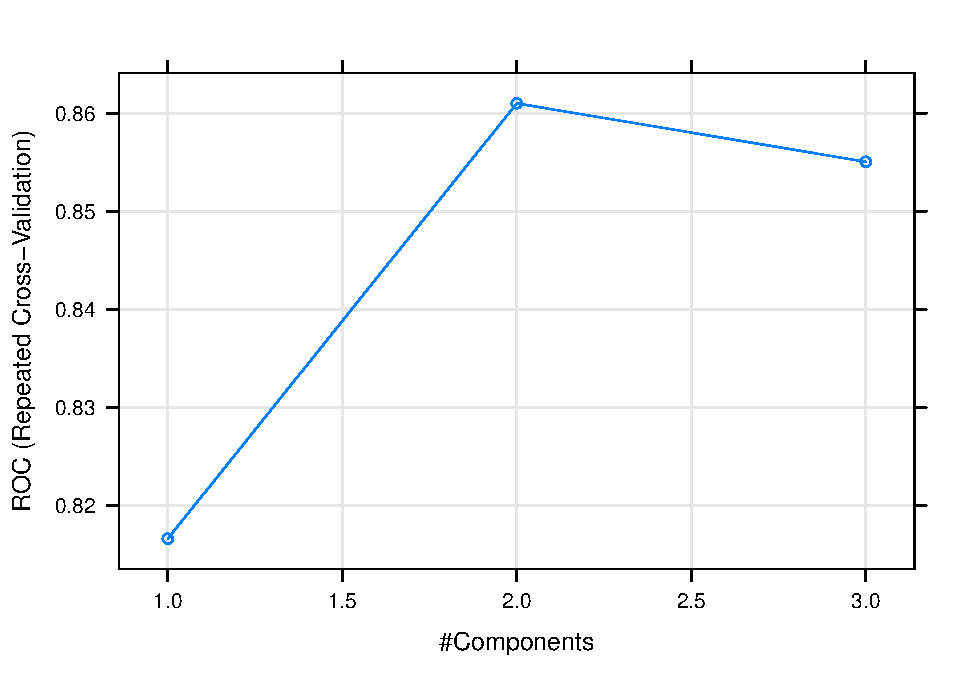
\includegraphics[width=0.7\linewidth]{tutorial_files/figure-latex/unnamed-chunk-11-1} \end{center}

\begin{Shaded}
\begin{Highlighting}[]
\NormalTok{plsFit3x10cv <-}\StringTok{ }\KeywordTok{train}\NormalTok{ (Class }\OperatorTok{~}\StringTok{ }\NormalTok{., }\DataTypeTok{data=}\NormalTok{training, }\DataTypeTok{method=}\StringTok{"pls"}\NormalTok{, }\DataTypeTok{trControl=}\NormalTok{ctrl, }
                       \DataTypeTok{metric=}\StringTok{"ROC"}\NormalTok{, }
                       \DataTypeTok{tuneLength=}\DecValTok{15}\NormalTok{, }
                       \DataTypeTok{preProc=}\KeywordTok{c}\NormalTok{(}\StringTok{"center"}\NormalTok{,}\StringTok{"scale"}\NormalTok{))}
\NormalTok{plsFit3x10cv}
\end{Highlighting}
\end{Shaded}

\begin{verbatim}
## Partial Least Squares 
## 
## 157 samples
##  60 predictor
##   2 classes: 'M', 'R' 
## 
## Pre-processing: centered (60), scaled (60) 
## Resampling: Cross-Validated (10 fold, repeated 3 times) 
## Summary of sample sizes: 141, 141, 142, 141, 142, 141, ... 
## Resampling results across tuning parameters:
## 
##   ncomp  ROC        Sens       Spec     
##    1     0.8074487  0.7449074  0.7202381
##    2     0.8458416  0.7449074  0.7815476
##    3     0.8523562  0.7842593  0.7589286
##    4     0.8469577  0.8000000  0.7357143
##    5     0.8188657  0.7689815  0.7333333
##    6     0.7963542  0.7574074  0.7017857
##    7     0.7985780  0.7481481  0.7000000
##    8     0.8017030  0.7467593  0.7107143
##    9     0.7965360  0.7439815  0.7208333
##   10     0.7938988  0.7393519  0.7202381
##   11     0.7931134  0.7319444  0.7291667
##   12     0.7919147  0.7208333  0.7244048
##   13     0.7864914  0.7212963  0.7339286
##   14     0.7785384  0.7175926  0.7244048
##   15     0.7809276  0.7175926  0.7345238
## 
## ROC was used to select the optimal model using the largest value.
## The final value used for the model was ncomp = 3.
\end{verbatim}

\begin{Shaded}
\begin{Highlighting}[]
\KeywordTok{plot}\NormalTok{(plsFit3x10cv)}
\end{Highlighting}
\end{Shaded}

\begin{center}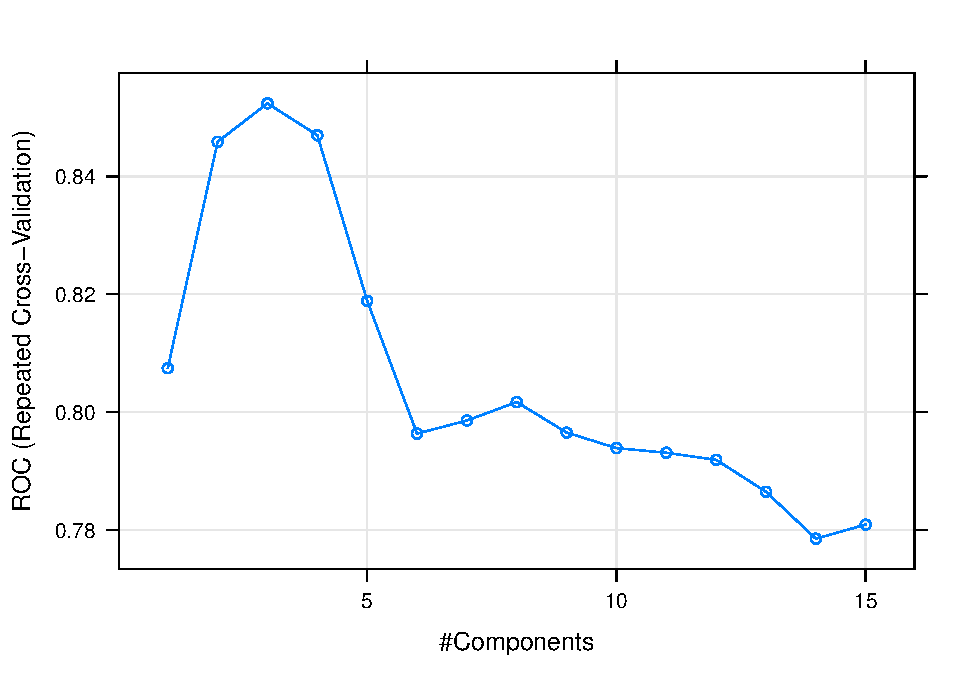
\includegraphics[width=0.7\linewidth]{tutorial_files/figure-latex/unnamed-chunk-11-2} \end{center}

Para predecir la clase de casos futuros, \textbf{caret} tendrá en cuenta
el clasificador con el mejor valor de sus parámetros. Consulta los
parámetros de la llamada a la función \textbf{predict} en
\href{https://www.rdocumentation.org/packages/caret/versions/6.0-72/topics/extractPrediction}{este
enlace}: entre éstos, la opción \textbf{type} merece ser estudiada. Con
la opción \textbf{probs} se calcula, por caso de test, la probabilidad
a-posteriori para cada valor de la clase; nos quedamos con la opción
\textbf{raw}, para el caso de test, con el valor de la variable clase
con mayor probabilidad a-posteriori. A partir de esta segunda opción
podemos calcular la matriz de confusión y la colección de estadísticos
de evaluación asociados; al fin y al cabo esto supone ``cruzar'', para
el caso de test, los valores de clase predichos con los valores de clase
reales.

\begin{Shaded}
\begin{Highlighting}[]
\NormalTok{plsProbs <-}\StringTok{ }\KeywordTok{predict}\NormalTok{(plsFit3x10cv, }\DataTypeTok{newdata =}\NormalTok{ testing, }\DataTypeTok{type =} \StringTok{"prob"}\NormalTok{)}
\NormalTok{plsClasses <-}\StringTok{ }\KeywordTok{predict}\NormalTok{(plsFit3x10cv, }\DataTypeTok{newdata =}\NormalTok{ testing, }\DataTypeTok{type =} \StringTok{"raw"}\NormalTok{)}
\KeywordTok{confusionMatrix}\NormalTok{(}\DataTypeTok{data=}\NormalTok{plsClasses, testing}\OperatorTok{$}\NormalTok{Class)}
\end{Highlighting}
\end{Shaded}

\begin{verbatim}
## Confusion Matrix and Statistics
## 
##           Reference
## Prediction  M  R
##          M 21  7
##          R  6 17
##                                           
##                Accuracy : 0.7451          
##                  95% CI : (0.6037, 0.8567)
##     No Information Rate : 0.5294          
##     P-Value [Acc > NIR] : 0.001311        
##                                           
##                   Kappa : 0.4872          
##                                           
##  Mcnemar's Test P-Value : 1.000000        
##                                           
##             Sensitivity : 0.7778          
##             Specificity : 0.7083          
##          Pos Pred Value : 0.7500          
##          Neg Pred Value : 0.7391          
##              Prevalence : 0.5294          
##          Detection Rate : 0.4118          
##    Detection Prevalence : 0.5490          
##       Balanced Accuracy : 0.7431          
##                                           
##        'Positive' Class : M               
## 
\end{verbatim}

A continuación, realizaremos una comparativa en base a los resultados de
evaluación interna de 3x10cv entre LDA y PLSDA. Ya que no hemos cambiado
la semilla de aleatorización, las particiones (de casos de training)
utilizadas en los procesos de ``resampling''-validación de cada
clasificador han sido las mismas: esto es, las ``folds''-hojas del
proceso de validación cruzada han sido las mismas en ambos
clasificadores.

\begin{Shaded}
\begin{Highlighting}[]
\NormalTok{resamps =}\StringTok{ }\KeywordTok{resamples}\NormalTok{(}\KeywordTok{list}\NormalTok{(}\DataTypeTok{pls=}\NormalTok{plsFit3x10cv, }\DataTypeTok{lda=}\NormalTok{ldaModel3x10cv))}
\KeywordTok{summary}\NormalTok{(resamps)}
\end{Highlighting}
\end{Shaded}

\begin{verbatim}
## 
## Call:
## summary.resamples(object = resamps)
## 
## Models: pls, lda 
## Number of resamples: 30 
## 
## ROC 
##          Min.   1st Qu.    Median      Mean   3rd Qu.     Max. NA's
## pls 0.6785714 0.7743056 0.8492063 0.8523562 0.9345238 1.000000    0
## lda 0.5714286 0.6651786 0.7648810 0.7620370 0.8377976 0.952381    0
## 
## Sens 
##      Min.   1st Qu.    Median      Mean   3rd Qu. Max. NA's
## pls 0.375 0.6666667 0.7777778 0.7842593 0.8854167    1    0
## lda 0.250 0.6250000 0.7500000 0.7189815 0.8506944    1    0
## 
## Spec 
##          Min.   1st Qu.    Median      Mean   3rd Qu. Max. NA's
## pls 0.4285714 0.6473214 0.7321429 0.7589286 0.8750000    1    0
## lda 0.2857143 0.5714286 0.7142857 0.6958333 0.8571429    1    0
\end{verbatim}

\begin{Shaded}
\begin{Highlighting}[]
\KeywordTok{xyplot}\NormalTok{(resamps, }\DataTypeTok{what=}\StringTok{"BlandAltman"}\NormalTok{)}
\end{Highlighting}
\end{Shaded}

\begin{center}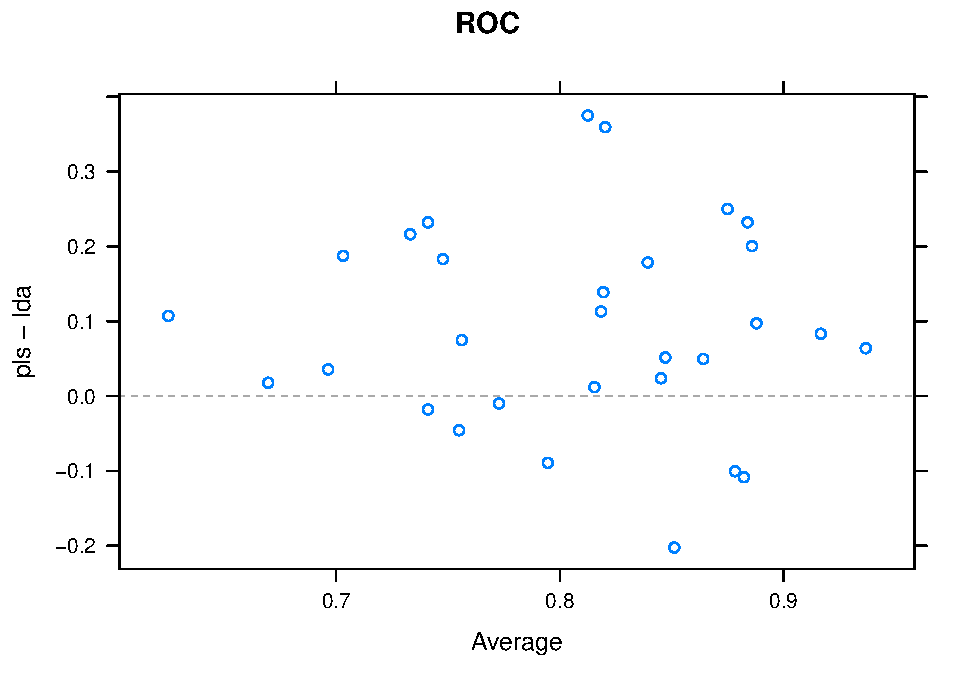
\includegraphics[width=0.7\linewidth]{tutorial_files/figure-latex/unnamed-chunk-14-1} \end{center}

\begin{Shaded}
\begin{Highlighting}[]
\NormalTok{diffs <-}\StringTok{ }\KeywordTok{diff}\NormalTok{(resamps)}
\KeywordTok{summary}\NormalTok{(diffs)}
\end{Highlighting}
\end{Shaded}

\begin{verbatim}
## 
## Call:
## summary.diff.resamples(object = diffs)
## 
## p-value adjustment: bonferroni 
## Upper diagonal: estimates of the difference
## Lower diagonal: p-value for H0: difference = 0
## 
## ROC 
##     pls     lda    
## pls         0.09032
## lda 0.00103        
## 
## Sens 
##     pls    lda    
## pls        0.06528
## lda 0.1083        
## 
## Spec 
##     pls    lda   
## pls        0.0631
## lda 0.1553
\end{verbatim}

Al compartir las ``folds''-hojas, un \emph{t-test} pareado calculará la
significancia de las diferencias entre los estimadores de error de ambos
modelos. El output de la comparativa contiene, para cada medida (área
bajo la curva ROC, sensibilidad y especifidad), la diferencia de medias
(positiva o negativa) entre clasificadores (siguiendo el orden de la
llamada a la función \textbf{resamps}); y el \emph{p-value} asociado
para interpretar el nivel de significatividad de las diferencias entre
los modelos.

Finalmente, se trata de chequear las diferencias, para cada score, entre
el par de clasificadores comparado. Y de interpretar, mediante el
\emph{p-value} asociado, si estas diferencias son estadísticamente
significativas o no,
\url{https://en.wikipedia.org/wiki/Statistical_significance}, usando el
clásico umbral de 0.05 a 0.10.

\end{document}
